\subsection{Traffic Manager}

\includegraphics[width=0.9\linewidth]{../../img/frontend.pdf}

Sitting between the key-value store accelerator and the NIC is the traffic
manager, which routes network packets between the accelerator and the CPU.

Packets from the network card are first written into the main buffer.
At the same time, the controller inspects the packet header to determine if
the packet is an IPv4 UDP packet and that the payload is a Memcached binary
GET request. A memcached GET request looks like the following.

\begin{center}
    \begin{tabular}{|c|c|c|c|c|}
        \hline
          & 0 & 1 & 2 & 3 \\
        \hline
        0 & \multicolumn{2}{|c}{Request ID} & \multicolumn{2}{|c|}{Sequence Num} \\
        \hline
        4 & \multicolumn{2}{|c|}{\# Datagrams} & 0x00 & 0x00 \\
        \hline
        8 & 0x80 & 0x00 & \multicolumn{2}{c|}{Key Length} \\
        \hline
        12 & \multicolumn{4}{|c|}{Zeros} \\
        \hline
        16 & \multicolumn{4}{|c|}{Total Body Length} \\
        \hline
        20 & \multicolumn{4}{|c|}{\multirow{3}{*}{Zeros}} \\
        \cline{1-1}
        24 & \multicolumn{4}{|c|}{} \\
        \cline{1-1}
        28 & \multicolumn{4}{|c|}{} \\
        \hline
        32 & \multicolumn{4}{|c|}{Key} \\
        ... & \multicolumn{4}{|c|}{} \\
        \hline
    \end{tabular}
\end{center}

The first eight octets are a pseudo-TCP header which is used by memcached to
match requests and responses. We only ever use single-packet messages,
so the sequence number is always zero and the number of datagrams is 
always one. The controller saves the request ID (as well as MAC addresses
from the ethernet header, IP addresses from the IP header, and port numbers
from the UDP header) to use in constructing the response packet.
Bytes 8 - 31 are the memcached binary protocol headers. The first byte is a
magic value 0x80, which indicates that the packet is a memcached request
(as opposed to a response). The second byte is an opcode 0x00, indicating that
it is a GET request. The other important fields are the key length and total
body length, which should be the same. Bytes 32 and on are the key.

If the packet does not contain a GET request, the packet
is sent on to the DMA engine, which will transfer the packet to the CPU.
If it is a GET packet, the key is sent to the accelerator and
the packet is moved from the main buffer to a defer buffer, allowing the
traffic manager to process subsequent packets without waiting for the result
to come back from the accelerator.

If a result does come back, the deferred packet is removed from the buffer and
the responder unit constructs a response by adding the necessary headers and
computing the IP and UDP checksums. The response is then sent back to the NIC.
A memcached binary GET response should look like the following

\begin{center}
    \begin{tabular}{|c|c|c|c|c|}
        \hline
          & 0 & 1 & 2 & 3 \\
        \hline
        0 & \multicolumn{2}{|c}{Request ID} & \multicolumn{2}{|c|}{Sequence Num} \\
        \hline
        4 & \multicolumn{2}{|c|}{\# Datagrams} & 0x00 & 0x00 \\
        \hline
        8 & 0x81 & 0x00 & \multicolumn{2}{c|}{0x0000} \\
        \hline
        12 & 0x04 & \multicolumn{3}{c|}{Zeros} \\
        \hline
        16 & \multicolumn{4}{|c|}{Total Body Length} \\
        \hline
        20 & \multicolumn{4}{|c|}{\multirow{2}{*}{Zeros}} \\
        \cline{1-1}
        24 & \multicolumn{4}{|c|}{} \\
        \hline
        28 & \multicolumn{4}{|c|}{0x00000001} \\
        \hline
        32 & \multicolumn{4}{|c|}{0xdeadbeef} \\
        \hline
        36 & \multicolumn{4}{|c|}{Value} \\
        ... & \multicolumn{4}{|c|}{} \\
        \hline
    \end{tabular}
\end{center}

As before, the first eight bytes are a pseudo-TCP header. The request ID here
should be the same as the request ID of the corresponding request.
The binary protocol header starts with the magic number 0x81, indicating a
response, followed by the opcode 0x00, indicating a response to a GET request.
The response body begins with a 4-byte extras section containing the bytes
DEADBEEF. The total body length should thus be set to the length of the value
plus four. The rest of the body is the value.

If a zero-length result is returned, indicating that the key was not found in
the accelerator, the deferred packet is sent on to the DMA engine.

The traffic manager also takes outbound packets from the DMA engine. An arbiter
is used to interleave transmission of these packets with transmission of
memcached response packets from the accelerator.
